\pdfminorversion=4
\documentclass[aspectratio=169]{beamer}

\mode<presentation>
{
  \usetheme{default}
  \usecolortheme{default}
  \usefonttheme{default}
  \setbeamertemplate{navigation symbols}{}
  \setbeamertemplate{caption}[numbered]
  \setbeamertemplate{footline}[frame number]  % or "page number"
  \setbeamercolor{frametitle}{fg=white}
  \setbeamercolor{footline}{fg=black}
} 

\usepackage[english]{babel}
\usepackage[utf8x]{inputenc}
\usepackage{tikz}
\usepackage{courier}
\usepackage{array}
\usepackage{bold-extra}
\usepackage{minted}
\usepackage[thicklines]{cancel}
\usepackage{fancyvrb}

\xdefinecolor{dianablue}{rgb}{0.18,0.24,0.31}
\xdefinecolor{darkblue}{rgb}{0.1,0.1,0.7}
\xdefinecolor{darkgreen}{rgb}{0,0.5,0}
\xdefinecolor{darkgrey}{rgb}{0.35,0.35,0.35}
\xdefinecolor{darkorange}{rgb}{0.8,0.5,0}
\xdefinecolor{darkred}{rgb}{0.7,0,0}
\definecolor{darkgreen}{rgb}{0,0.6,0}
\definecolor{mauve}{rgb}{0.58,0,0.82}

\title[2018-09-24-dianahep-histbook]{histbook (and histogramming in Python in general)}
\author{Jim Pivarski}
\institute{Princeton University -- DIANA-HEP}
\date{September 24, 2018}

\usetikzlibrary{shapes.callouts}

\begin{document}

\logo{\pgfputat{\pgfxy(0.11, 7.4)}{\pgfbox[right,base]{\tikz{\filldraw[fill=dianablue, draw=none] (0 cm, 0 cm) rectangle (50 cm, 1 cm);}\mbox{\hspace{-8 cm}
\includegraphics[height=1 cm]{princeton-logo-long.png}
\includegraphics[height=1 cm]{diana-hep-logo-long.png}}}}}

\begin{frame}
  \titlepage
\end{frame}

\logo{\pgfputat{\pgfxy(0.11, 7.4)}{\pgfbox[right,base]{\tikz{\filldraw[fill=dianablue, draw=none] (0 cm, 0 cm) rectangle (50 cm, 1 cm);}\mbox{\hspace{-8 cm}
\includegraphics[height=1 cm]{princeton-logo.png}
\includegraphics[height=1 cm]{diana-hep-logo.png}}}}}

% Uncomment these lines for an automatically generated outline.
%\begin{frame}{Outline}
%  \tableofcontents
%\end{frame}

% START START START START START START START START START START START START START

\begin{frame}{Histogramming in Python}
\scriptsize
\begin{tabular}{c l c p{2.5 cm} p{1 cm} p{4 cm}}
$\surd$ & \href{https://pypi.python.org/pypi/histogram}{\textcolor{blue}{histogram}} & 2011 & conventional-HEP & Numpy & Numpy, Matplotlib, HDF5 \\
$\surd$ & \href{https://pypi.python.org/pypi/pyhistogram}{\textcolor{blue}{pyhistogram}} & 2014 & conventional-HEP & Numpy & Numpy, Matplotlib, datetime \\
$\surd$ & \href{https://pypi.python.org/pypi/histogramy}{\textcolor{blue}{histogramy}} & & & & \\
$\surd$ & \href{https://pypi.python.org/pypi/pypeaks}{\textcolor{blue}{pypeaks}} & & & & \\
$\surd$ & \href{https://pypi.python.org/pypi/SimpleHist}{\textcolor{blue}{SimpleHist}} & & & & \\
$\surd$ & \href{https://pypi.python.org/pypi/hierogram}{\textcolor{blue}{hierogram}} & & & & \\
$\surd$ & \href{https://pypi.python.org/pypi/histo}{\textcolor{blue}{histo}} & & & & \\
$\surd$ & \href{https://pypi.python.org/pypi/python-metrics}{\textcolor{blue}{python-metrics}} & & & & \\
$\surd$ & \href{https://pypi.python.org/pypi/statscounter}{\textcolor{blue}{statscounter}} & & & & \\
$\surd$ & \href{https://pypi.python.org/pypi/multihist}{\textcolor{blue}{multihist}} & & & & \\
$\surd$ & \href{https://pypi.python.org/pypi/vaex}{\textcolor{blue}{vaex}} & & & & \\
$\surd$ & \href{https://pypi.python.org/pypi/datagram}{\textcolor{blue}{datagram}} & & & & \\
$\surd$ & \href{https://pypi.python.org/pypi/hdrhistogram}{\textcolor{blue}{hdrhistogram}} & & & & \\
$\surd$ & \href{http://www.ifh.de/~middell/dashi/index.html}{\textcolor{blue}{dashi}} & & & & \\
$\surd$ & \href{https://pypi.python.org/pypi/physt}{\textcolor{blue}{physt}} & & & & \\
$\surd$ & \href{https://github.com/ibab/matplotlib-hep}{\textcolor{blue}{matplotlib-hep}} & & & & \\
& \href{https://github.com/theodoregoetz/histogram}{\textcolor{blue}{theodoregoetz}} & & & & \\
$\surd$ & \href{https://pypi.org/project/paida}{\textcolor{blue}{paida}} & & & \\
$\surd$ & \href{https://pypi.org/project/rootpy}{\textcolor{blue}{rootpy}} & & & & \\
& \href{https://pypi.org/project/root_numpy}{\textcolor{blue}{root\_numpy}} & & & & \\
& \href{https://yoda.hepforge.org/pydoc}{\textcolor{blue}{YODA}} & & & & \\
& \href{https://root.cern.ch/pyroot}{\textcolor{blue}{PyROOT}} & & & & \\
\end{tabular}
\end{frame}


%% \begin{frame}{Another histogram package?}
%% \large
%% \vspace{0.5 cm}
%% \begin{columns}
%% \column{1.05\linewidth}
%% Histograms are easy to implement, and because they're so essential to HEP analysis, it's worth optimizing the design and experimenting with new ones.

%% \vspace{0.5 cm}
%% \textcolor{darkblue}{Is there a downside to creating new histogram packages?}

%% \Large
%% \vspace{0.2 cm}
%% \begin{center}
%% \uncover<2->{Interoperability?}
%% \end{center}

%% \large
%% \vspace{0.2 cm}
%% \uncover<3->{If Alice uses ROOT, Bob uses Yoda, Claire uses AIDA, and Donald uses Numpy, how are they going to collaborate on analysis?}
%% \end{columns}
%% \end{frame}

%% \begin{frame}[fragile]{Interoperability doesn't have to be hard}
%% \large
%% \vspace{0.25 cm}
%% As long as we're talking about a handful of standards, we can synchronize them.

%% \begin{columns}
%% \column{0.5\linewidth}
%% \small
%% \vspace{-0.5 cm}
%% \begin{minted}{python}
%% import uproot  # >= 3.0.2
%% import numpy
%% f = uproot.recreate("some.root")
%% f["myhist"] = numpy.histogram(
%%     numpy.random.normal(0, 1, 10000))


%% import ROOT
%% f = ROOT.TFile("some.root")
%% h = f.Get("myhist")
%% h.Draw()
%% \end{minted}
%% \column{0.4\linewidth}
%% \hfill 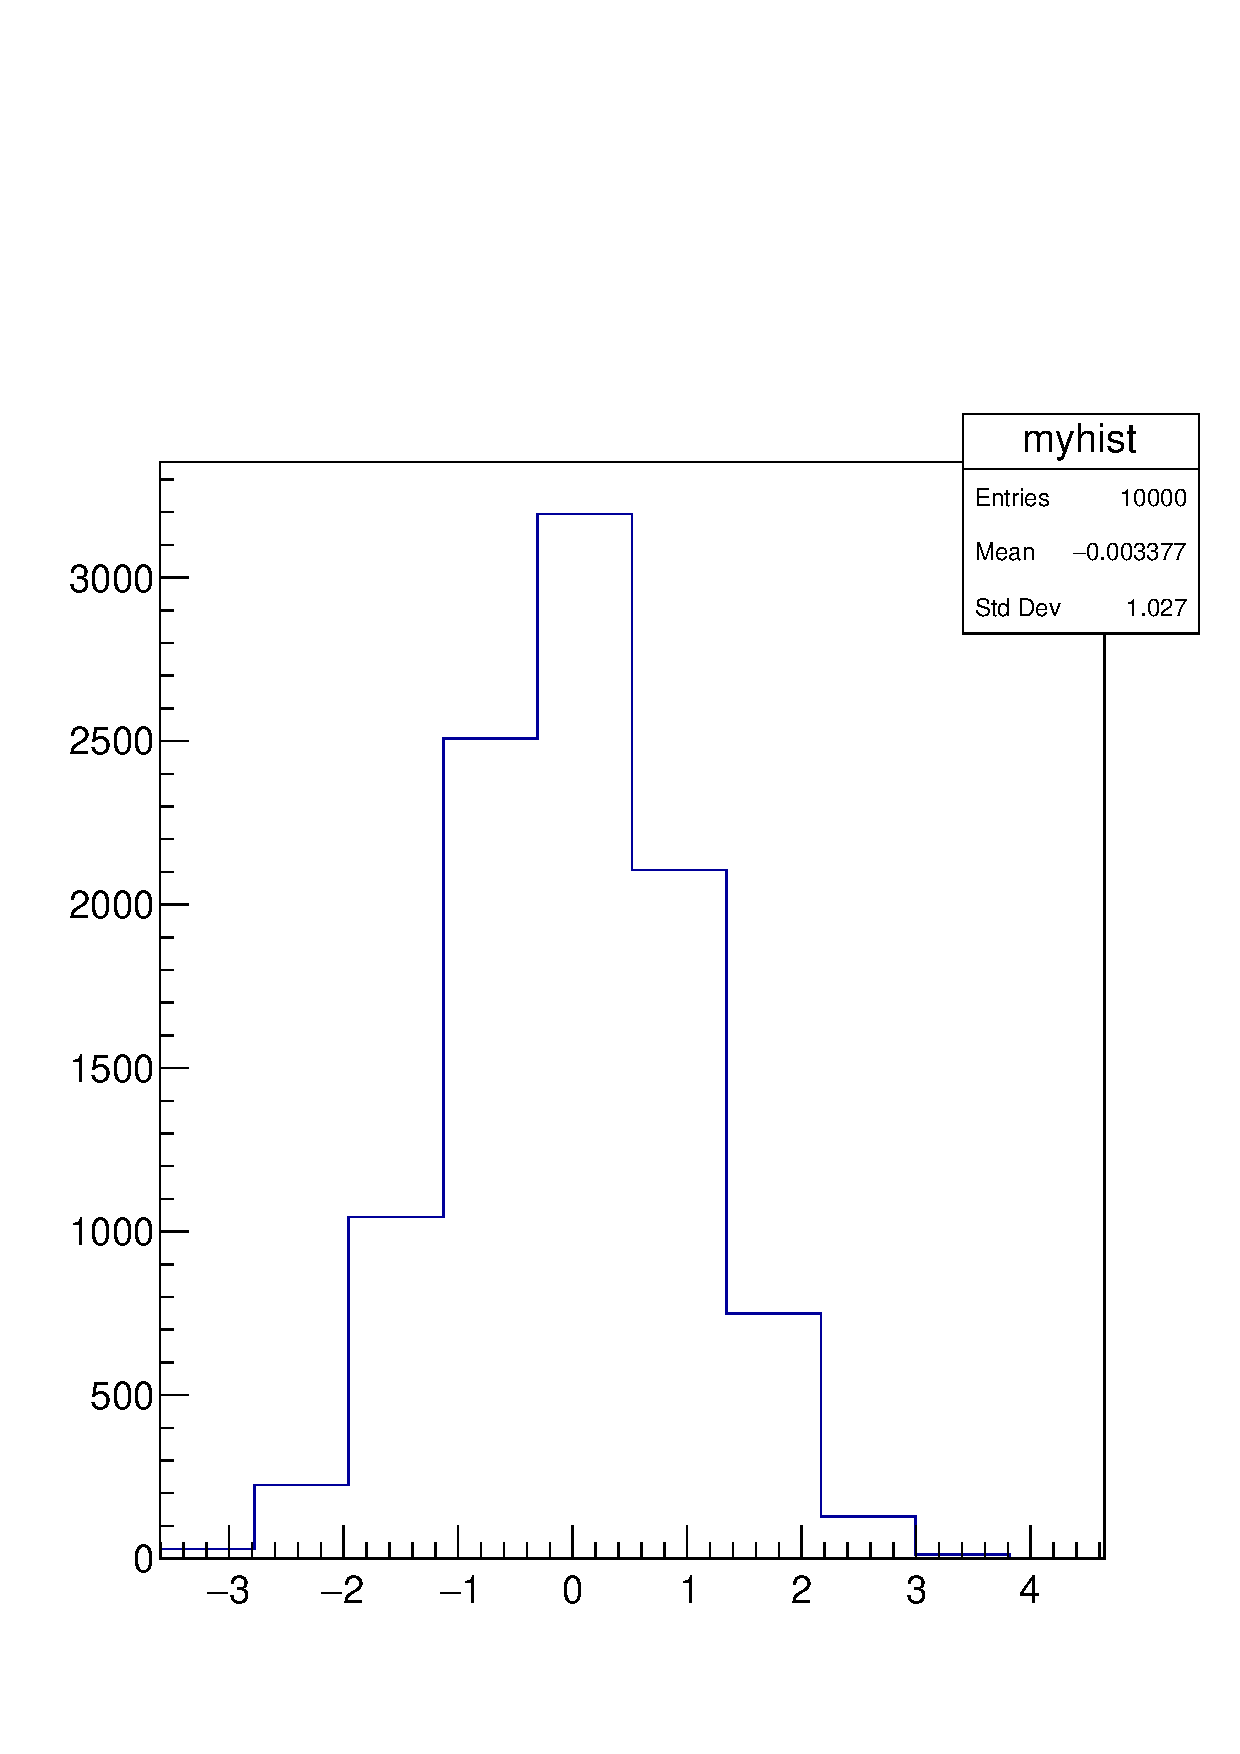
\includegraphics[width=\linewidth]{numpy-to-root.pdf}
%% \end{columns}

%% \large
%% Pratyush Das's histogram-writing feature $+$ a straightforward Numpy translation.
%% \end{frame}

%% \begin{frame}{Commonality}
%% \large
%% \vspace{0.5 cm}
%% All histograms have
%% \begin{itemize}
%% \item A way of describing edges (regular numbins/low/high or irregular edges)
%% \item Number of entries in each bin, possibly weighted
%% \end{itemize}

%% \vspace{0.5 cm}
%% Some histograms have
%% \begin{itemize}
%% \item Weighted bin errors (\mintinline{python}{sumw2})
%% \item Global number of entries, mean, standard deviation, other statistics\ldots
%% \item Titles, labels, metadata\ldots
%% \item Plotting options, overlay curves\ldots
%% \end{itemize}

%% \vspace{0.5 cm}
%% Translations among standards may be lossy in the optional features, but not in the essential features.
%% \end{frame}

%% \begin{frame}{}
%% \large
%% \vspace{0.5 cm}
%% \mintinline{python}{numpy.histogram} is absolutely minimal: a 2-tuple of edges and bin contents.

%% \normalsize
%% \vspace{0.5 cm}
%% Alternatives:
%% \begin{description}
%% \item[pip:] rootpy:  \hfill (HEP)
%% \item[pip:] qhist \hfill (HEP)
%% \item[pip:] fast-histogram \hfill (astronomy)
%% \item[pip:] SimpleHist \hfill (synchrotron radiation)
%% \item[pip:] pyhistogram \hfill (heavy ions)
%% \item[pip:] histogram \hfill (neutron scattering)
%% \item[tarball:] Yoda \hfill (analysis preservation)
%% \end{description}

%% \item[pip:] physt \hfill ()




%% \end{frame}


\end{document}
